\documentclass[11pt,a4paper]{jarticle}
\usepackage[dvips]{graphicx}
\usepackage{here}

\title{{チーム研究\\実験計画}}
\date{2014年6月3日(火)}
\author{小森谷 大介、川畑 裕也、深津 佳智}

\begin{document}

\maketitle

%1
\section{概要}
昨年度の研究から得た知見を基に、表面及び背面に突起もしくはくぼみを付けた新たなケースのデザインを考える。
具体的には、スマートフォンの表面(タッチパネル)に突起を付けることにより、ユーザがタッチパネルにタッチする際の手がかりとするという発展案を考えた。
作成したプロトタイプ、及び、実験計画について報告する。

%2
\section{突起の位置}
突起の位置の候補として図\ref{fig:iti}の箇所が挙げられた。下記にそれぞれ理由とともに示す。
また突起の数は1つとする。
\begin{figure}[H]
  \begin{center}
  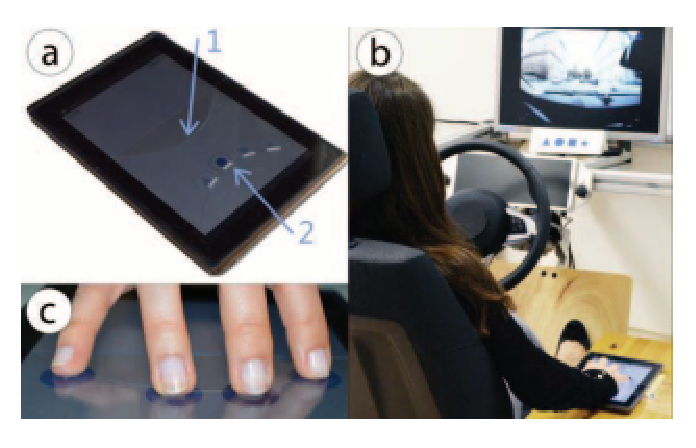
\includegraphics[width=8cm]{fig/figure1.eps}
  \caption{突起の位置候補}
  \label{fig:iti}
  \end{center}
\end{figure}

\begin{enumerate}
 \item[1.中央]\mbox{}\\
	端末を把持しているため画面端は認識可能である。中央に配置することにより、指の位置を正確に把握しやすくなる可能性がある。
 \item[2.左上]\mbox{}\\ 
	片手把持の時、ターゲットまで距離が遠く、昨年度の実験においてタッチ精度が悪かっため。
 \item[3.右下]\mbox{}\\
	片手把持の時、親指を極端に曲げなければならずタッチしにくい領域であるため。
 \item[4.右上]\mbox{}\\
	片手把持をした際、容易に親指を用いてタッチすることが可能な位置である。
 \item[5.左下]\mbox{}\\
	片手把持をした際、容易に親指を用いてタッチすることが可能な位置である。
 \item[6.左上端]\mbox{}\\
	片手把持をした際、もっとも遠くタッチしにくい領域である。端末の端とも近いため効果がどの程度でるのか不明。
\end{enumerate}



%3
\section{突起の位置の考察}
突起は中央点の他に左上、右下について作成することとなった。左上、右下の突起を作成する位置について考察を行った。


実験は3×3、4×4、5×5の条件においてタッチ操作を行う。そのため、突起は前述の3つの条件においてわかりやすい位置とならなければならない。3つの条件について以下の図\ref{fig:fig1}、\ref{fig:fig2}、\ref{fig:fig3}に示す。また、3つの条件をすべて重ねた図\ref{fig:fig4}を以下に示す。

\begin{figure}[H]
  \begin{center}
  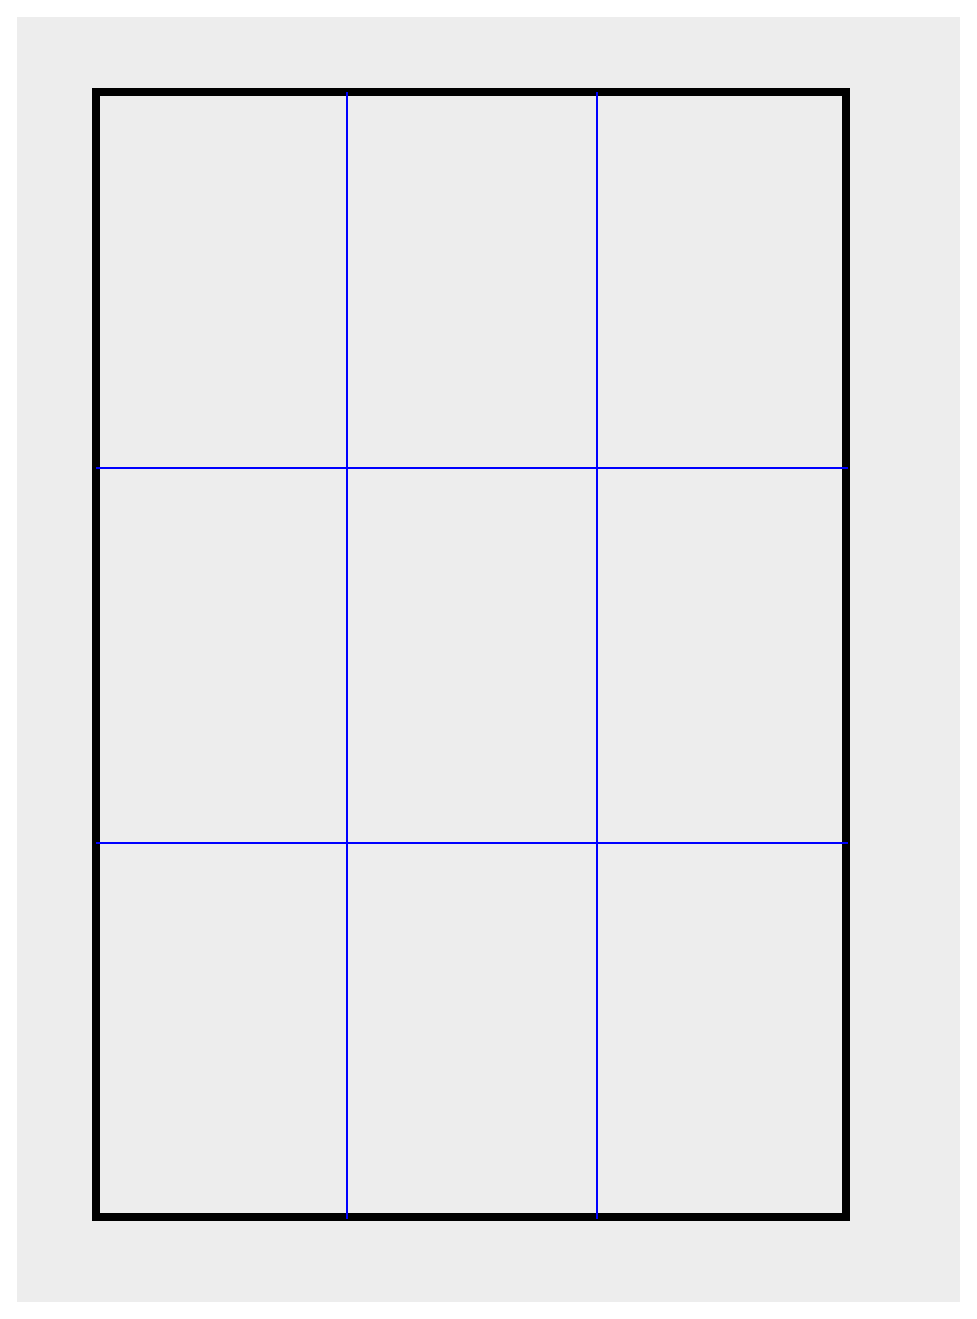
\includegraphics[width=4cm]{fig/photo1.eps}
  \caption{3×3}
  \label{fig:fig1}
  \end{center}
\end{figure}

\begin{figure}[H]
  \begin{center}
  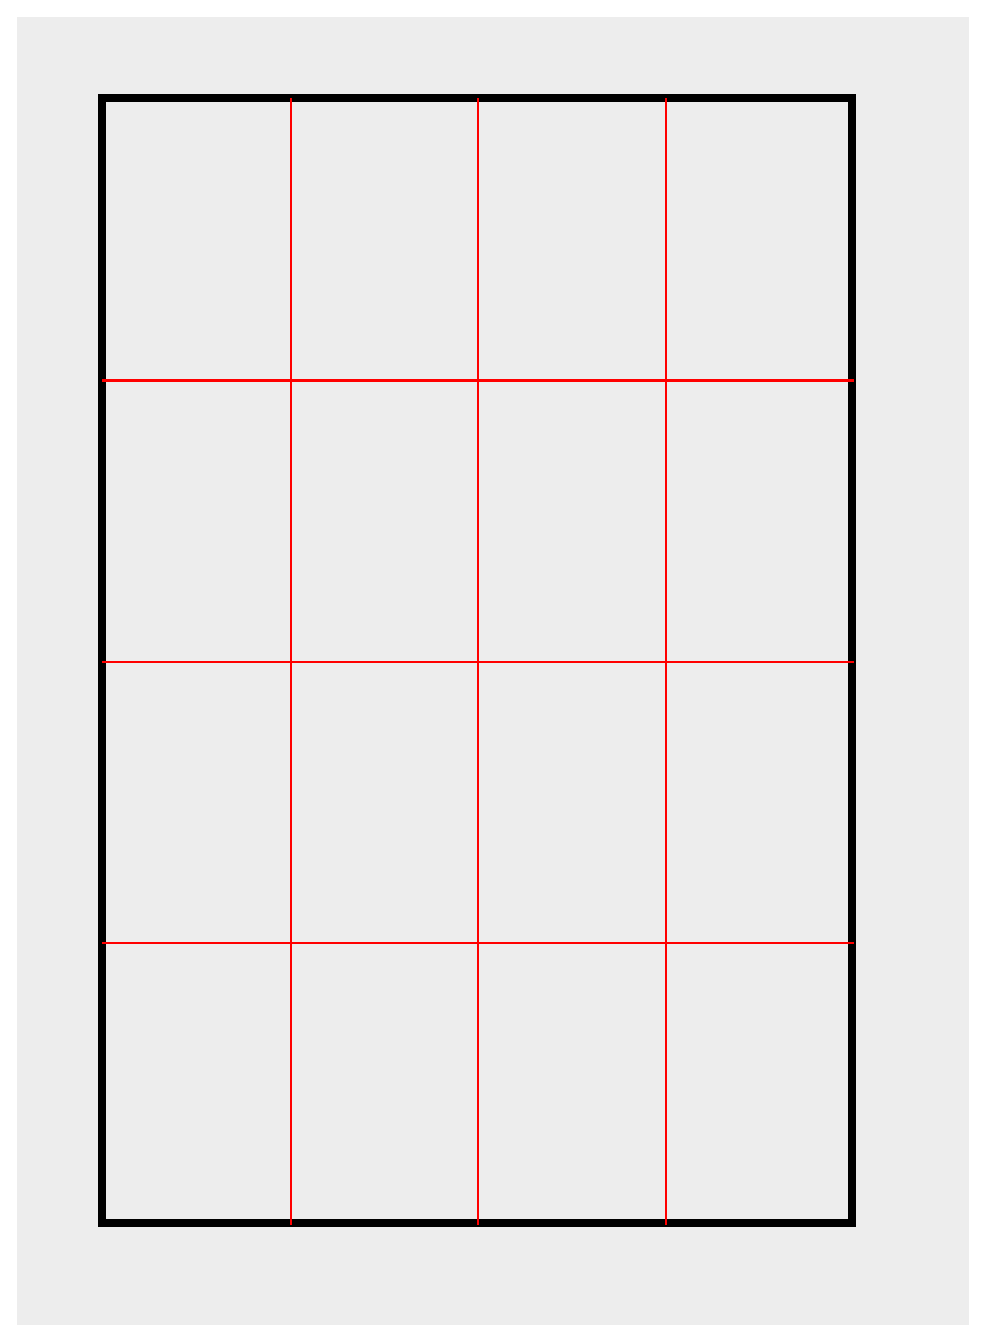
\includegraphics[width=4cm]{fig/photo2.eps}
  \caption{4×4}
  \label{fig:fig2}
  \end{center}
\end{figure}

\begin{figure}[H]
  \begin{center}
  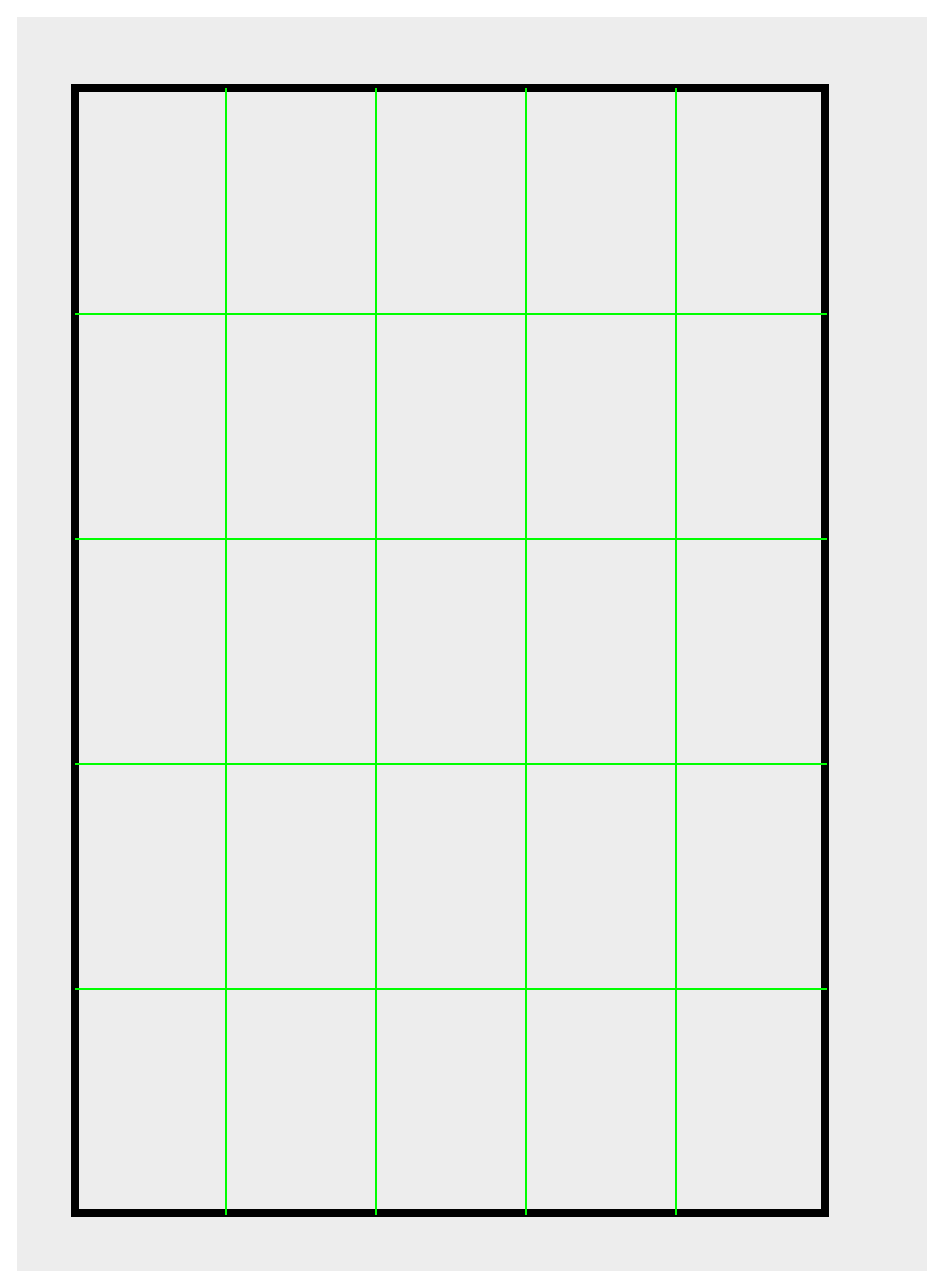
\includegraphics[width=4cm]{fig/photo3.eps}
  \caption{5×5}
  \label{fig:fig3}
  \end{center}
\end{figure}

\begin{figure}[H]
  \begin{center}
  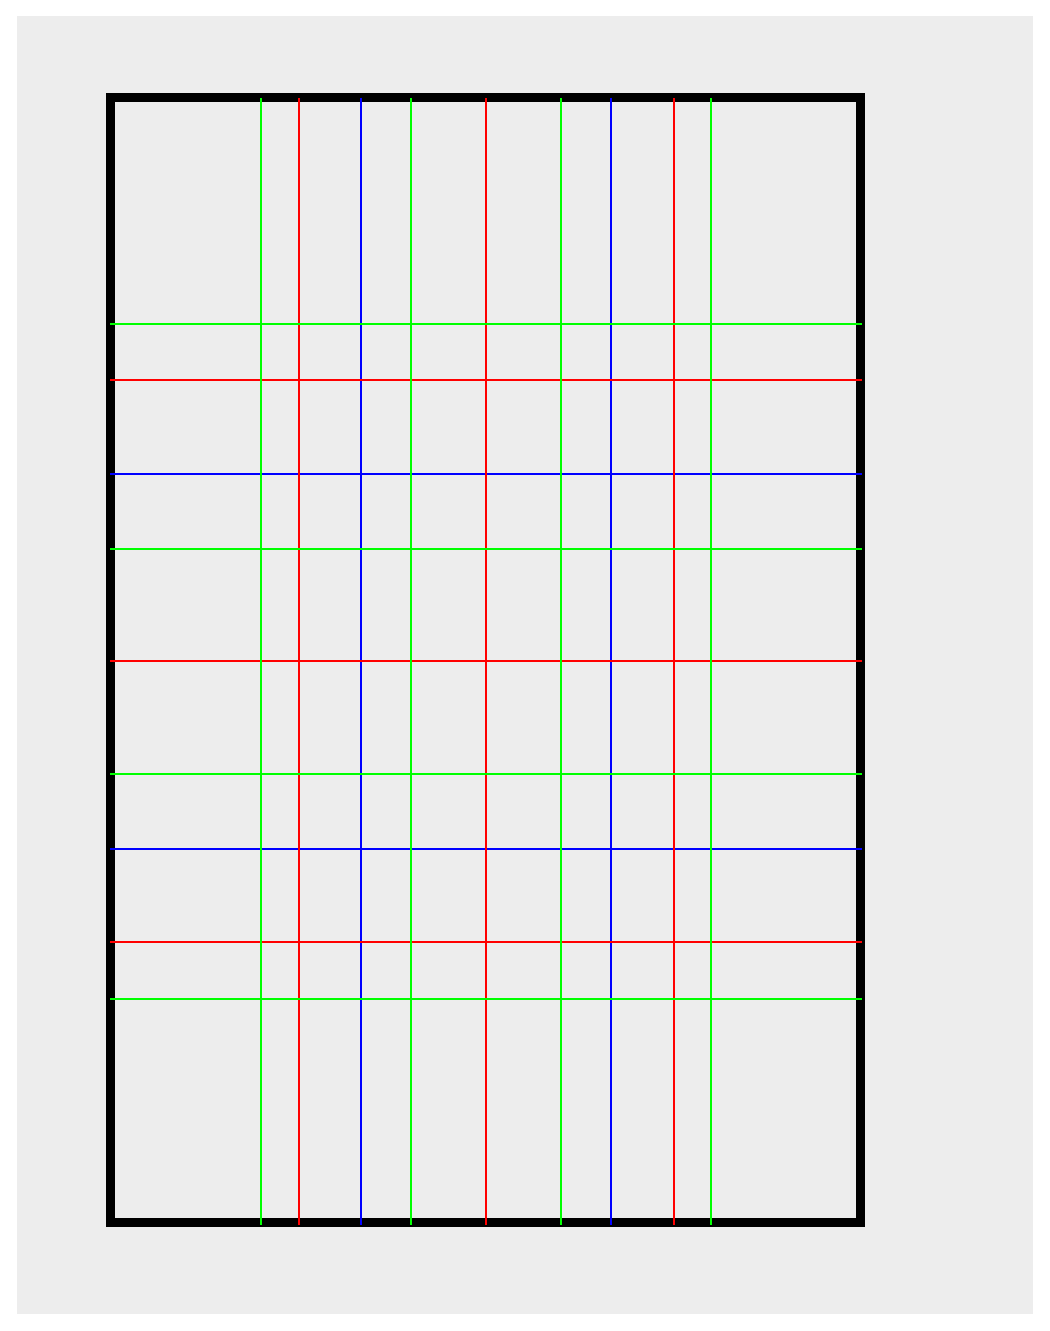
\includegraphics[width=4cm]{fig/photo4.eps}
  \caption{図\ref{fig:fig1}から図\ref{fig:fig3}までを重ねた}
  \label{fig:fig4}
  \end{center}
\end{figure}


図\ref{fig:fig4}からわかるように3つの条件において重なる点は存在しない。そこで、3条件のそれぞれの交点においてもっとも点が密集している点を取ることが良いのではないかと考えた。


3条件それぞれの交点において他の2条件の交点との距離を評価した。評価としては3×3と4×4、3×3と4×4、4×4と5×5の3つの組み合わせに置いてすべての交点同士の距離を計算することとした。これにより3条件すべてにおいてもっともホームポジションとして使いやすい点を計算出来るのではないかと考えた。


この評価の結果、図\ref{fig:fig5}に示す3点が3条件において最も接近している3点であることがわかった。よってこの3点から突起をつける点を選ぶことが適当であると考えられる。特に4×4の点(図\ref{fig:fig5}示した3点の中央)は3×3(図\ref{fig:fig5}示した3点の右下)と5×5図\ref{fig:fig5}示した3点の左上)の間にあるため評価実験における基準として使用できるのではないかと考えた。

\begin{figure}[H]
  \begin{center}
  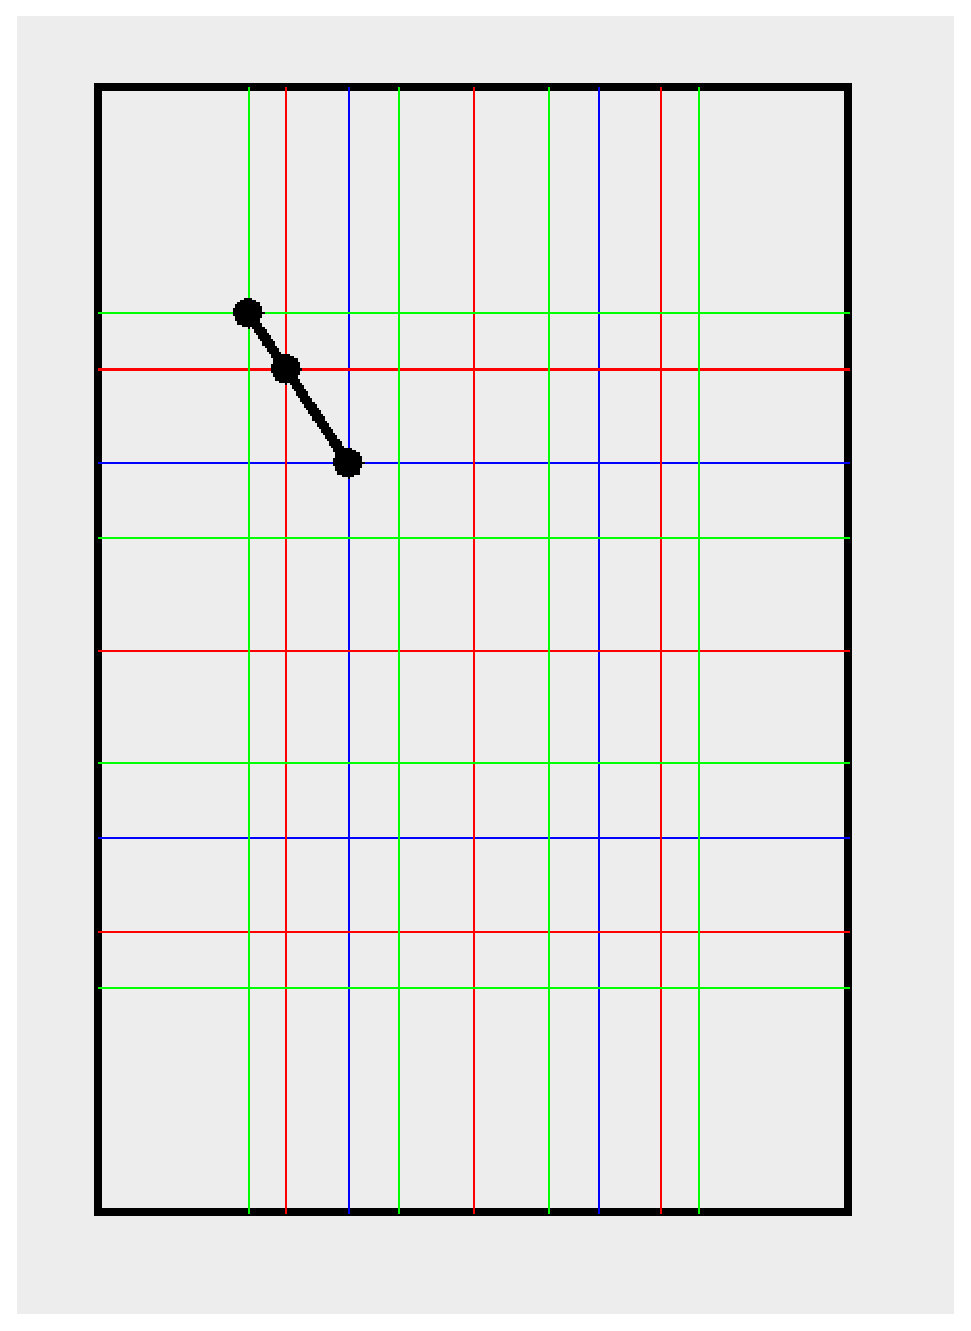
\includegraphics[width=4cm]{fig/photo5.eps}
  \caption{3条件で最も点において接近している3点}
  \label{fig:fig5}
  \end{center}
\end{figure}







\section{実験計画}
作成したプロトタイプを用いて、昨年度のソフトウェア科学会大会投稿時の実験と同様の実験を行うことを考えている。
具体的には、
\begin{itemize}
	\item 突起条件:突起無し条件、表面突起A地点条件、表面突起B条件、表面突起C地点、背面突起A地点条件、背面突起B条件、背面突起C地点
	\item 分割条件:3~$\times$~3分割条件、4~$\times$~4分割条件、5~$\times$~5分割条件
\end{itemize}
の2種類の実験条件を設定し、被験者にアイズフリーにおいてタッチパネル上のターゲットをタッチしてもらう実験を行うことを考えている。
昨年度の実験と今回の実験計画の相違点は、ケース条件であったところを突起条件に変え、表面及び背面の両方において実験を行う点である。
また、昨年度の実験においては開始点タッチ条件と終了点タッチ条件が存在したが、
表面に付いている突起をタッチの手がかりとできることを考え、終了点タッチ条件のみにした。(昨年度の実験では、開始点タッチ条件と終了点タッチ条件のタッチ精度に有意差は見られなかった)。

%4
\section{サーベイ}
深津さんの気まぐれにより

%5
\section{今後の予定}
7月に研究会かHISに出し、HCIIに出せるのが理想的なルート
%研究会とかHCIIとか書いておけば良いかと
\begin{itemize}
  \item 6月
  \begin{itemize}
    \item 実験
  \end{itemize}
  \item 7月
  \begin{itemize}
    \item HCI研究会(日程未定)
  \end{itemize}
  \item 8月
  \begin{itemize}
    \item 31日 HCIIアブスト締切(去年の日程)
  \end{itemize}
\end{itemize}
\bibliographystyle{jalpha}
\bibliography{shokunyu}
\end{document}
